% previous variable selection details file

\subsection{Normal Distributions Transformed to the Unit Simplex: The ALoVaS method. }\label{sec:ALN_chapter}

This chapter outlines the additive logistic transformation, which transforms a $d$ dimensional multivariate normal distribution onto the unit simplex in $d+1$ dimensions. Note that the unit simplex in $d+1$ dimensions actually lies in a subspace of $d$ dimensions because of the constraint that the sum of the probabilities equals one. 

The goal of this chapter is to find a transform that moves the space $\mathbb{R}^d$ \newnot{symbol:real} to the simplex $\mathbb{S}^d$. \newnot{symbol:simp} The simplex $\mathbb{S}^d$ is a space defined by the constraints $\{x_i: 0<x_i<1, \sum_{j=1}^dx_j <1 \}$, and the extra term $x_{d+1}=1-\sum_{j=1}^d x_j$ ensures the total sums to 1.  

Define the notation $\yvec$, for the normal random variables that reside in the $\Rsp{d}$  dimensional space. Define the notation $\xvec$  for the vector that resides on $\simp{d}$, the simplex in $d$ dimensions. We use an underline to indicate that the stated quantity is a column vector and capital greek letters (and $I$) will denote matrices (the identity matrix) 

\begin{equation}\label{eqn:simplex_transform}
x_i = \frac{e^{y_i}}{1+\displaystyle{\sum_{j=1}^de^{y_j}}}. \\
\end{equation}
The Jacobian of the transform is defined as
\newnot{symbol:jacobian}
\begin{equation}\label{eqn:jacobian}
J(\yvec \vert \xvec) = \left( \prod_{j=1}^{d+1}x_j \right)^{-1}.
\end{equation}

It is important to note that $\yvec\in\Rsp{d}$, whereas $\xvec\in\simp{d}$. The $d$ dimensional normal has the usual parameters and density

\begin{equation}\label{eqn:multinormal}
f_{\yvec}(\yvec\vert \Sigma, \mu)=(2\pi)^{-d/2}|\Sigma|^{-1/2}\exp{\left(-1/2(\yvec-\muvec)^T\Sigma^{-1}(\yvec-\muvec)\right)}.
\end{equation}

Upon applying the transformation defined by Equation \ref{eqn:simplex_transform}, we arrive at the additive logistic normal (ALN) distribution, with density 

\begin{equation}
f_{\xvec}(\xvec\vert \Sigma, \mu)=\frac{(2\pi)^{-d/2}}{\sqrt{\vert\Sigma\vert}\prod_{j=1}^{d+1}x_j } 
\exp{\left(-1/2(\text{log}(\xvec_{(d+1)}/x_{d+1})-\muvec)^T\Sigma^{-1}(\text{log}(\xvec_{(d+1)}/x_{d+1})-\muvec)\right)}.
\end{equation}
The vector notation $\xvec_{(d+1)}$ denotes the vector in $d$ dimensions that has the $d+1$ entry removed from the vector $\xvec$. 
It is important to note that this density function is defined on the space $\simp{d}$ and \emph{not} on the space $\Rsp{d}$. 

A useful property of this transform is that we can handle probabilities defined on the $d$ dimensional simplex while working with a normal distribution. This is a common and comfortable probability distribution for most statisticians and applied scientists.
We now wish to understand how the specification of the mean vector $\muvec$ and the covariance matrix $\Sigma$ impact the structure of the ALN density. From simulation we can formulate the following conclusions: 

\begin{itemize}
\item With $\Sigma=I$, increasing the mean vector in the positive direction in any one of the $d$ components individually corresponds to shifting density towards the corner of the simplex associated with that covariate. 
\item With $\Sigma=I$, increasing the mean vector in the negative in \emph{all} $d$ components corresponds to shifting density towards the $d+1$ corner of the simplex. 
\item Keeping $\muvec =\vec{0}$, adjusting any of the variances corresponds to shifting towards a projected space of $\simp{d}$. 
\item With $\muvec =\vec{0}$, making one variance small corresponds to the shifting density towards the median of the simplex associated with the remaining $d$ dimensions. 
\item Making the $\Sigma$ matrix approximately singular and moving $\muvec$ in the negative direction for all components places most of the probability density along the median of simplex associated with first $d$ dimensions. 
\item If $\Sigma = \text{Diag}(\sigma^2_j)$,\newnot{symbol:diag} as the $\sigma^2_j$ entries become smaller, the probabilities approach the CGM specification.    
\end{itemize}

Using the transformation defined in Equation \ref{eqn:simplex_transform} and the fact that it is relatively simple to simulate from the vector normal distribution, the ALN density can be simulated. 

\begin{figure}[ht]
\begin{minipage}[b]{0.45\linewidth}
\centering
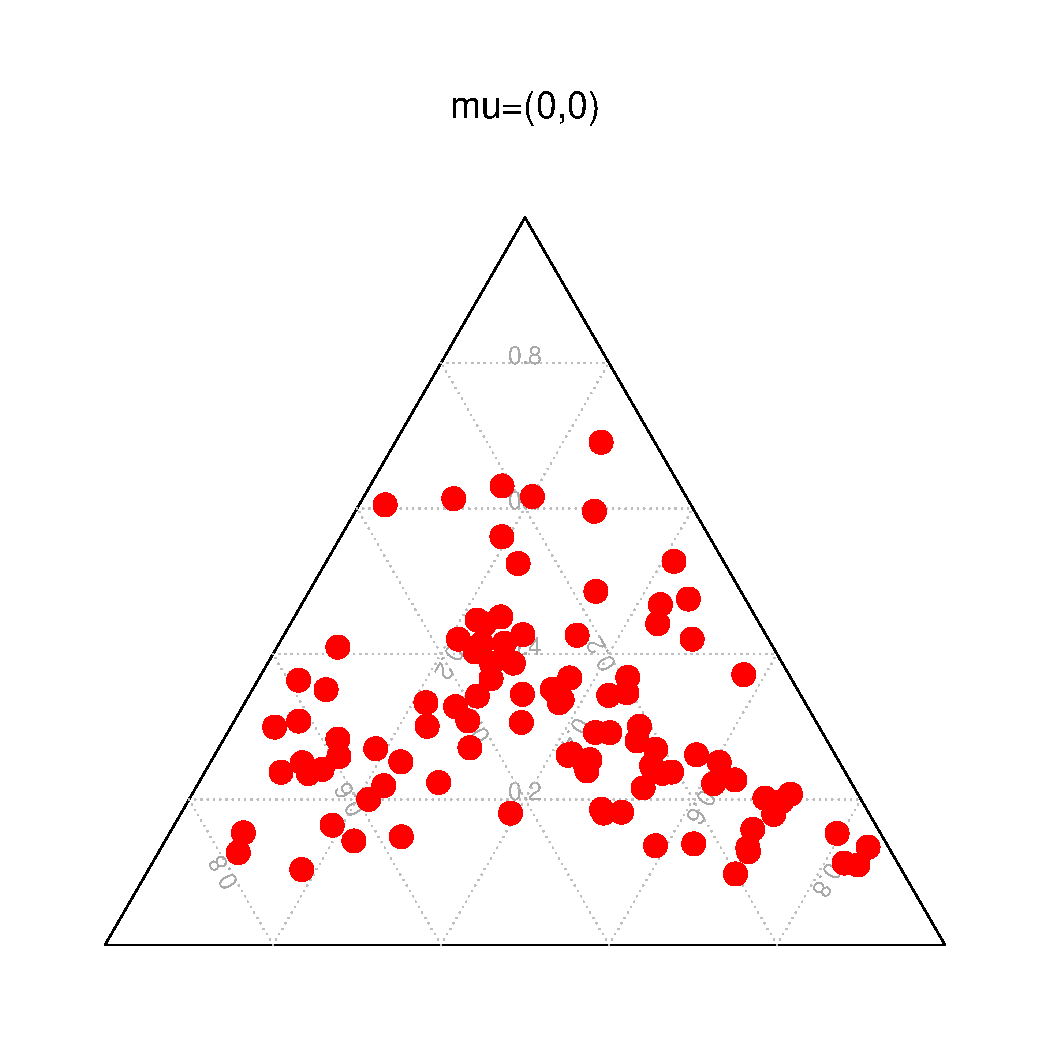
\includegraphics[width=\textwidth]{mu0_0.pdf}
\caption[ALN plot with a zero mean vector]{In this figure, $\muvec$ has all zero entries, with $\Sigma=I$, corresponding to the equiprobable case. Each probability is approximately $1/(d+1)$. }
\label{fig:figure9}
\end{minipage}
\hspace{0.5cm}
\begin{minipage}[b]{0.45\linewidth}
\centering
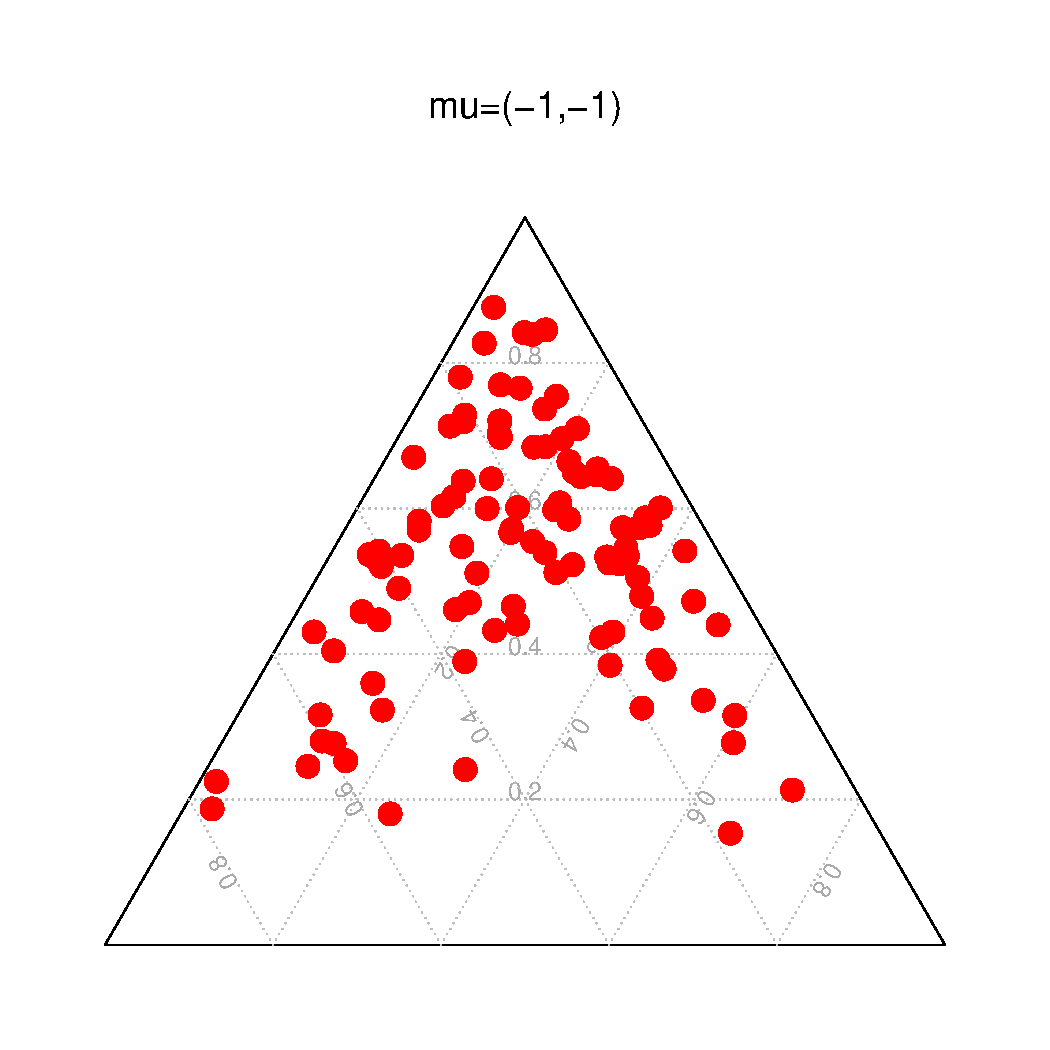
\includegraphics[width=\textwidth]{mu-1-1.pdf}
\caption[ALN plot with a negative one mean vector]{In this figure, $\vec{\mu}=(-1,-1)^T$, with $\Sigma=I$, corresponds to moving towards a sparser set of covariates. }
\label{fig:figure10}
\end{minipage}
\end{figure}

\begin{figure}[ht]
\begin{minipage}[b]{0.45\linewidth}
\centering
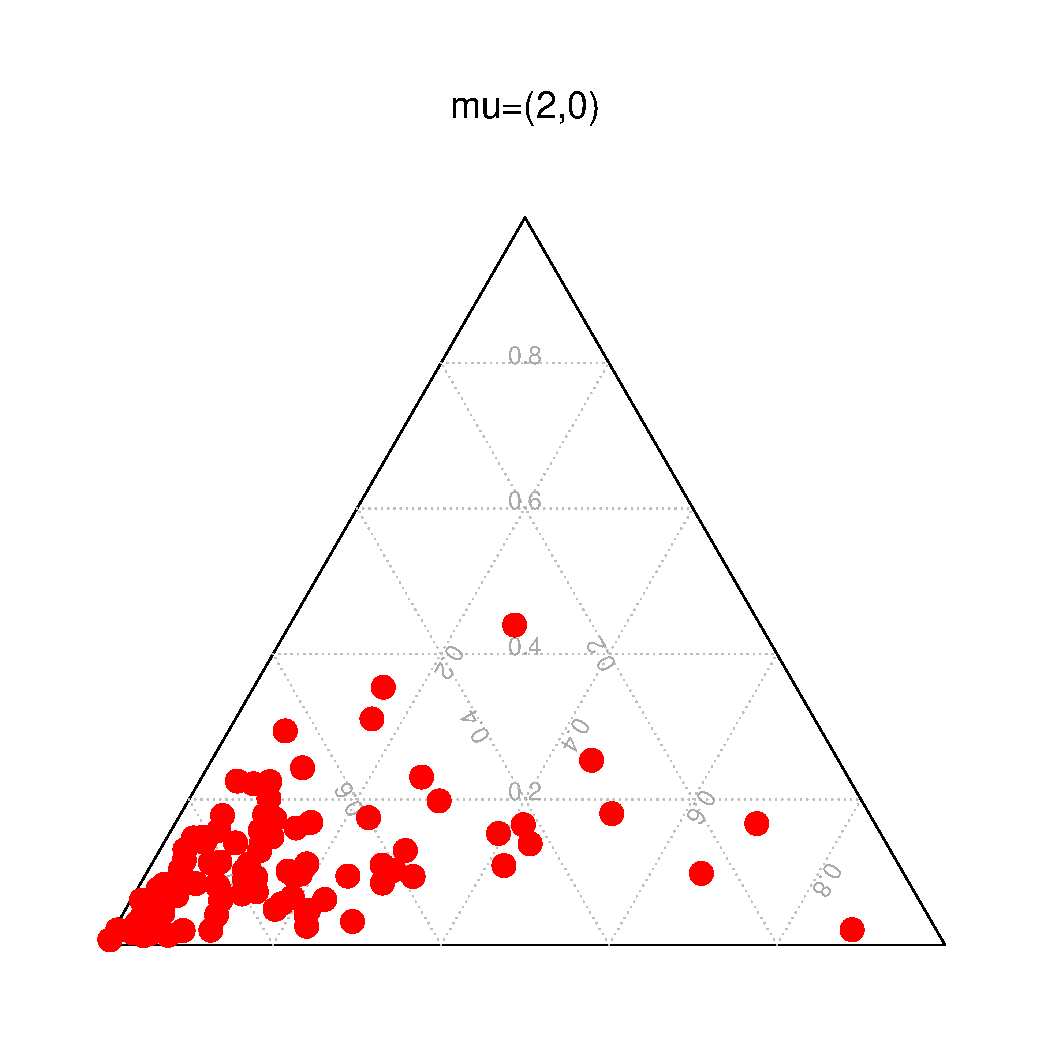
\includegraphics[width=\textwidth]{mu2_0.pdf}
\caption[ALN plot with a mean vector $(2,0)^{T}$]{$\vec{\mu}=(2,0)^T$, with $\Sigma=I$, moves the density towards one corner of the simplex. }
\label{fig:figure1}
\end{minipage}
\hspace{0.5cm}
\begin{minipage}[b]{0.45\linewidth}
\centering
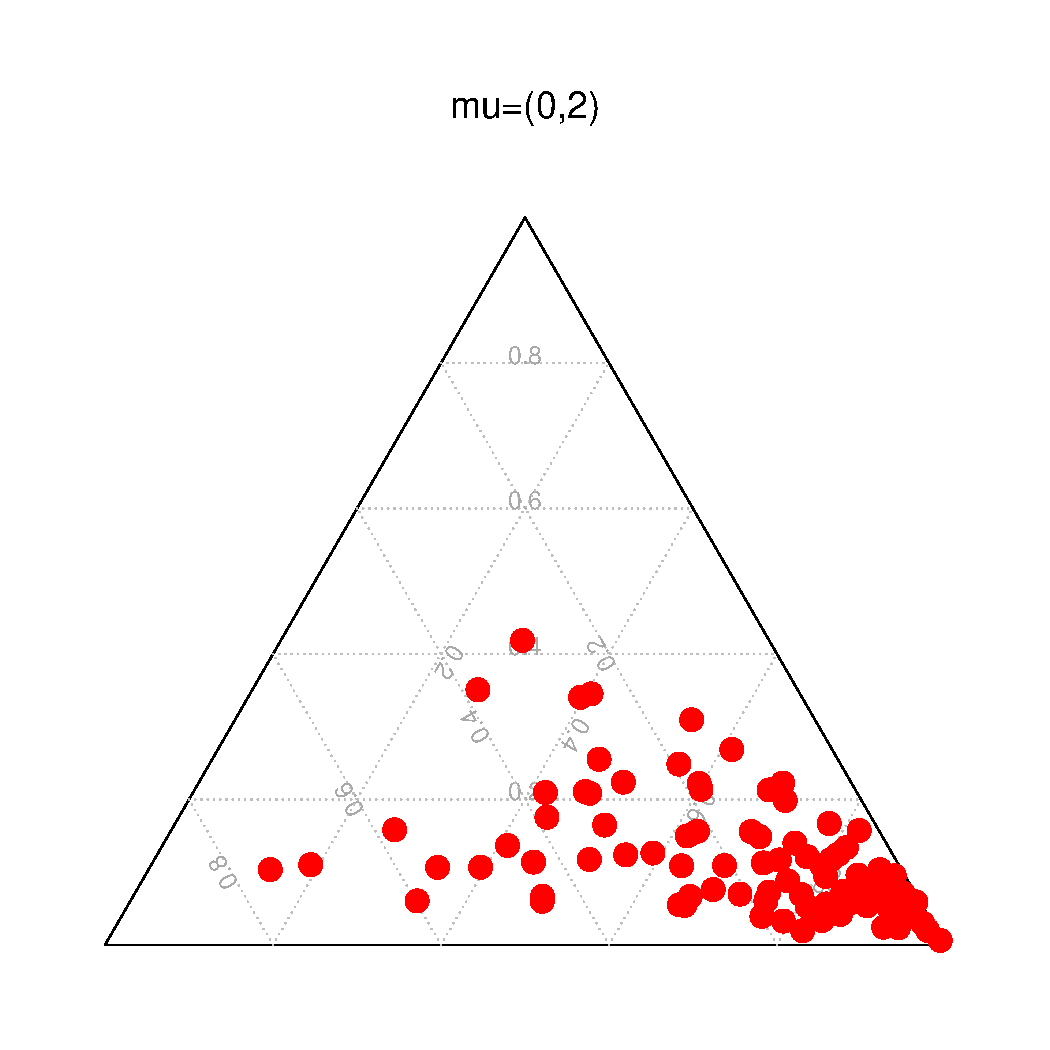
\includegraphics[width=\textwidth]{mu0_2.pdf}
\caption[ALN plot with mean vector $(2,0)^{T}$]{$\vec{\mu}=(0,2)^T$, with $\Sigma=I$, moves the density towards the other corner of the simplex. }
\label{fig:figur2}
\end{minipage}
\end{figure}

\begin{figure}[ht]
\begin{minipage}[b]{0.45\linewidth}
\centering
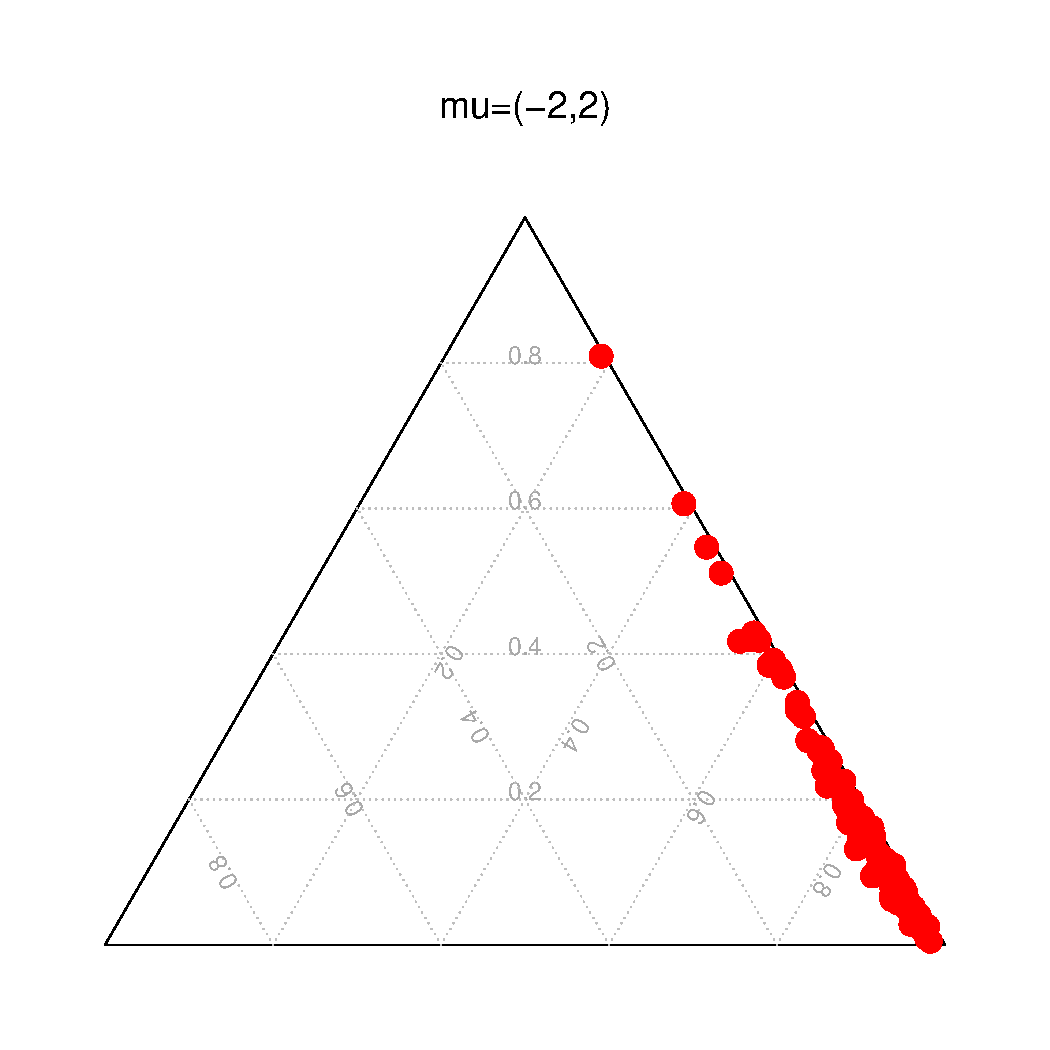
\includegraphics[width=\textwidth]{mu-2_2.pdf}
\caption[ALN plot with a mean vector of $(-2,2)^{T}$]{$\vec{\mu}=(-2,2)^T$, with $\Sigma=I$, corresponds to most probability mass along a corner of the simplex and is a sparse representation.} 
\label{fig:figure3}
\end{minipage}
\hspace{0.5cm}
\begin{minipage}[b]{0.45\linewidth}
\centering
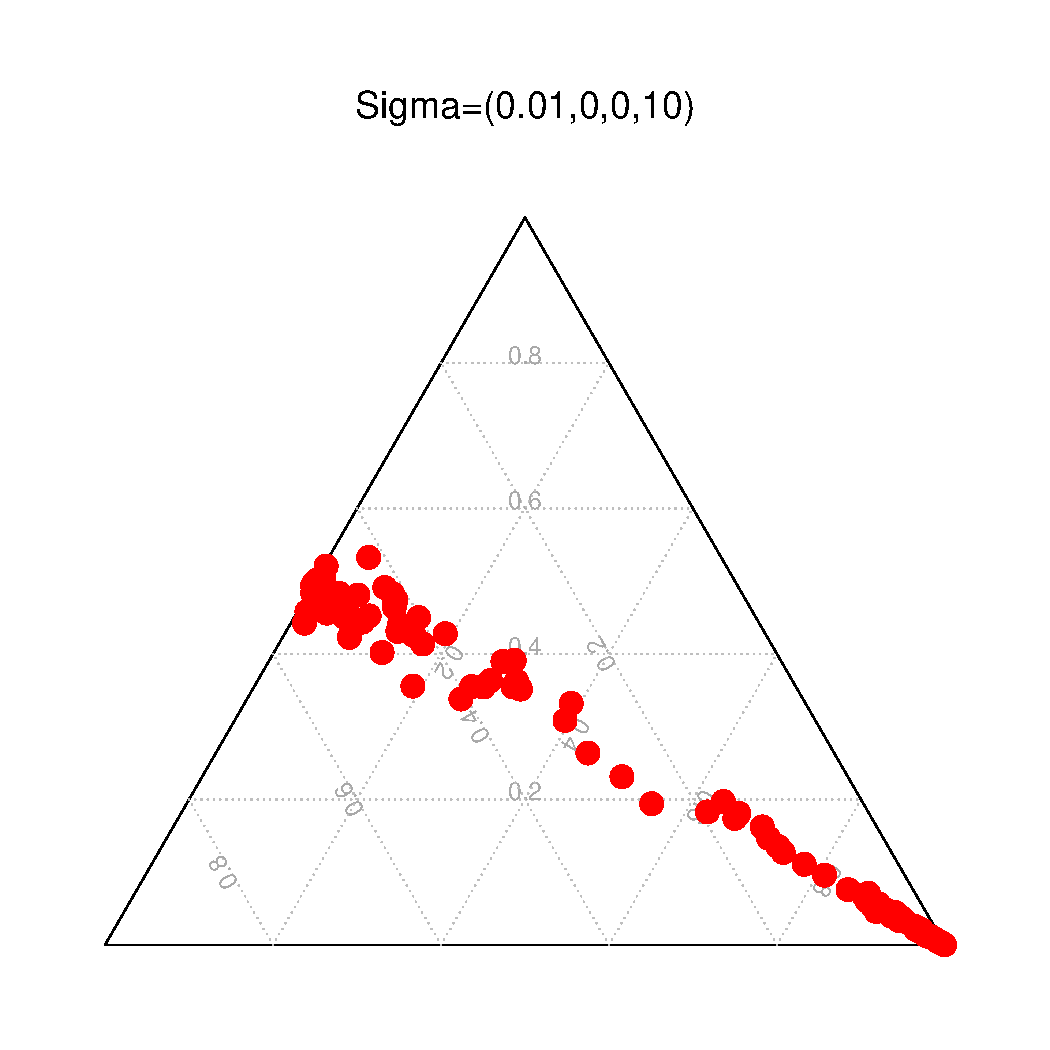
\includegraphics[width=\textwidth]{Sigma0_01_10.pdf}
\caption[ALN plot $\Sigma=\text{Diag(0.01,100)}$]{ $\vec{\mu}=\vec{0}$, with
 $\Sigma= \text{diag}(0.01, 100)$, corresponds to most density lying on a one dimensional subspace (the second covariate in the $\Rsp\ $ space).  }
\label{fig:figure4}
\end{minipage}
\end{figure}


\begin{figure}[ht]
\begin{minipage}[b]{0.45\linewidth}
\centering
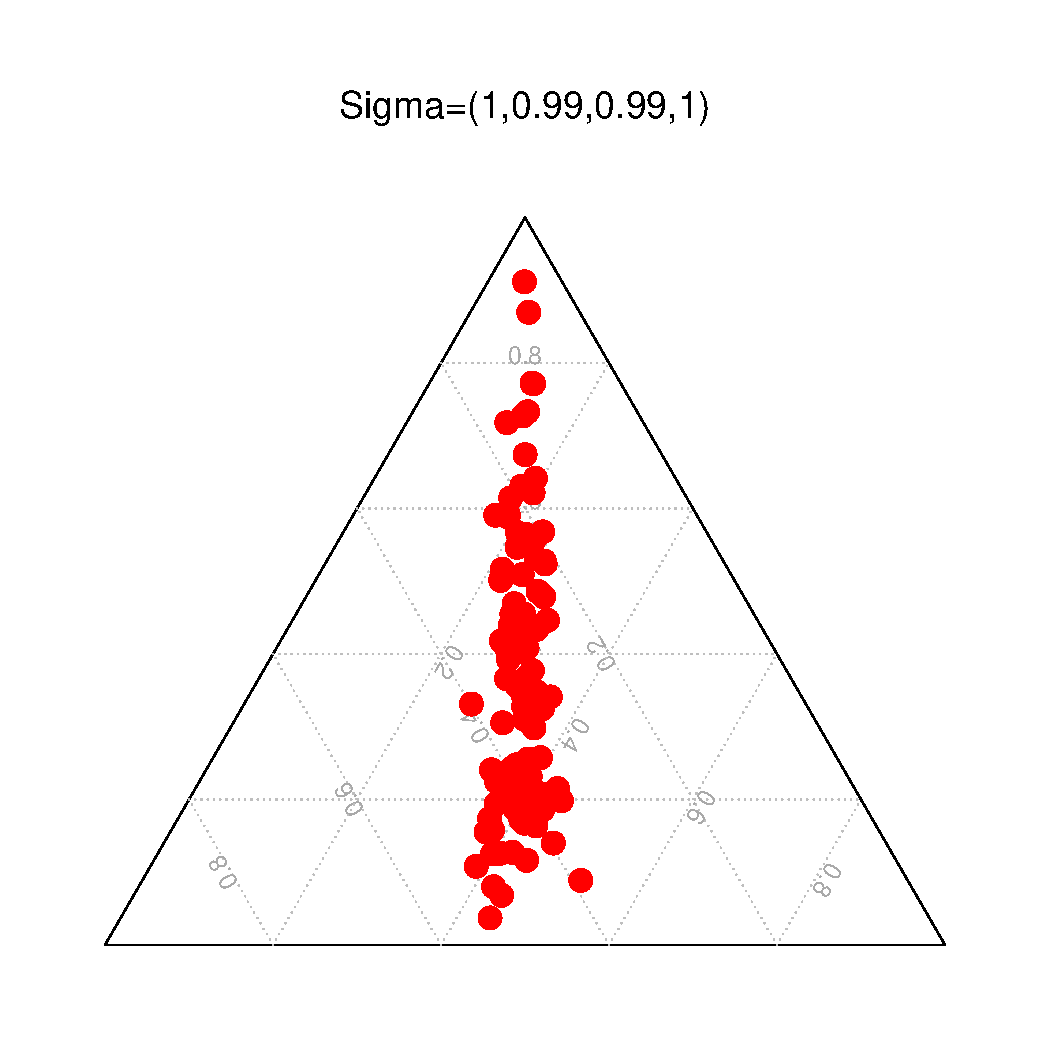
\includegraphics[width=\textwidth]{Sigma1_9_9_1.pdf}
\caption[ALN plot $\Sigma$ numerically singular]{Here $\Sigma$ is approximately singular and most of the probability mass in concentrated along the $d+1$th dimension in the $\mathbb{R}^{d+1}$ space.  }
\label{fig:figure5}
\end{minipage}
\hspace{0.5cm}
\begin{minipage}[b]{0.45\linewidth}
\centering
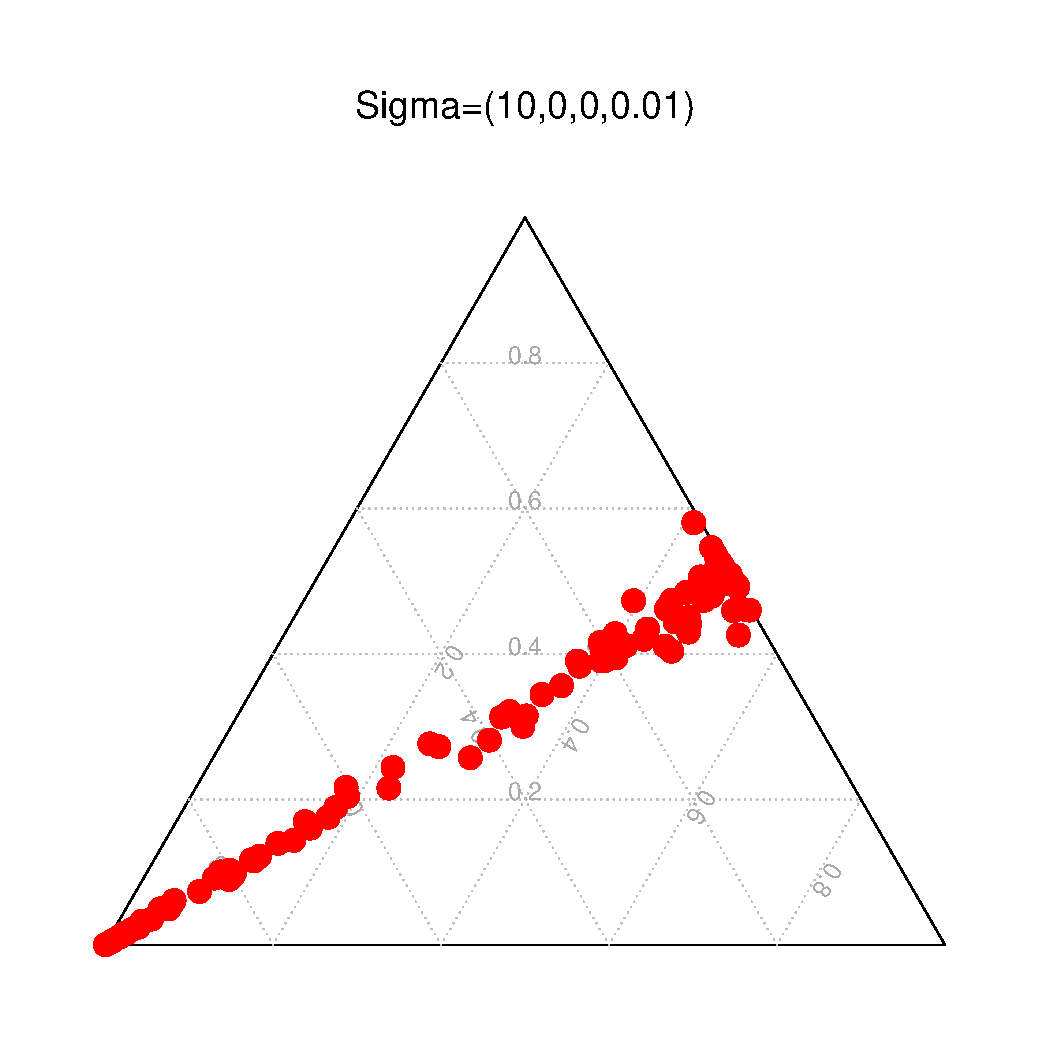
\includegraphics[width=\textwidth]{Sigma10_0_01.pdf}
\caption[Similar to the case in Figure \ref{fig:figure4} but with the variances reversed]{Similar to the case in Figure \ref{fig:figure4} but with the variances reversed.}
\label{fig:figure6}
\end{minipage}
\end{figure}

 \begin{figure}[ht]
\begin{minipage}[b]{0.45\linewidth}
\centering
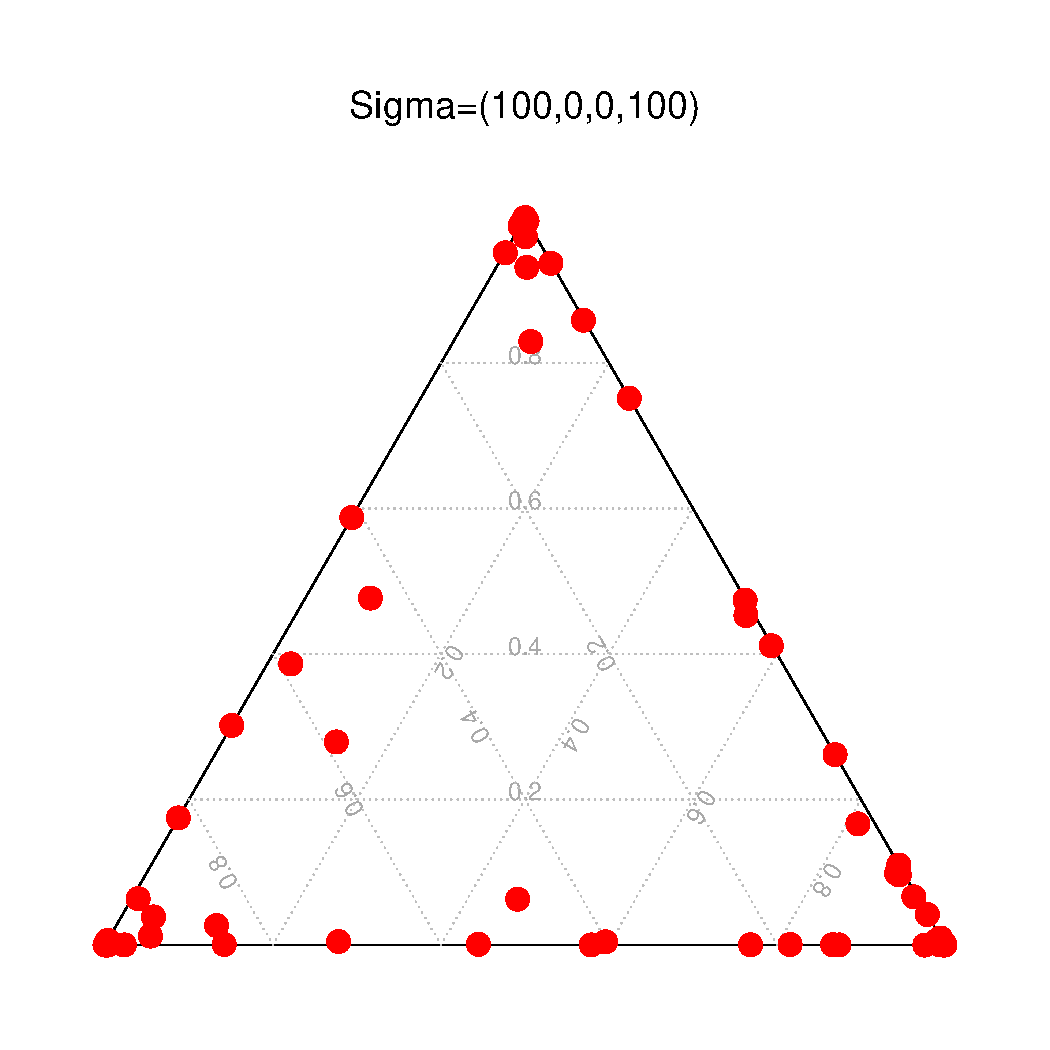
\includegraphics[width=\textwidth]{Sigma100_100.pdf}
\caption[ALN plot with a zero vector mean and $\Sigma=\text{Diag}(100,100)$]{$\vec{\mu}=\vec{0}$, with
 $\Sigma= \text{diag}(100, 100)$, corresponds to encouraging sparse representations \emph{a priori}.  }
\label{fig:figure7}
\end{minipage}
\hspace{0.5cm}
\begin{minipage}[b]{0.45\linewidth}
\centering
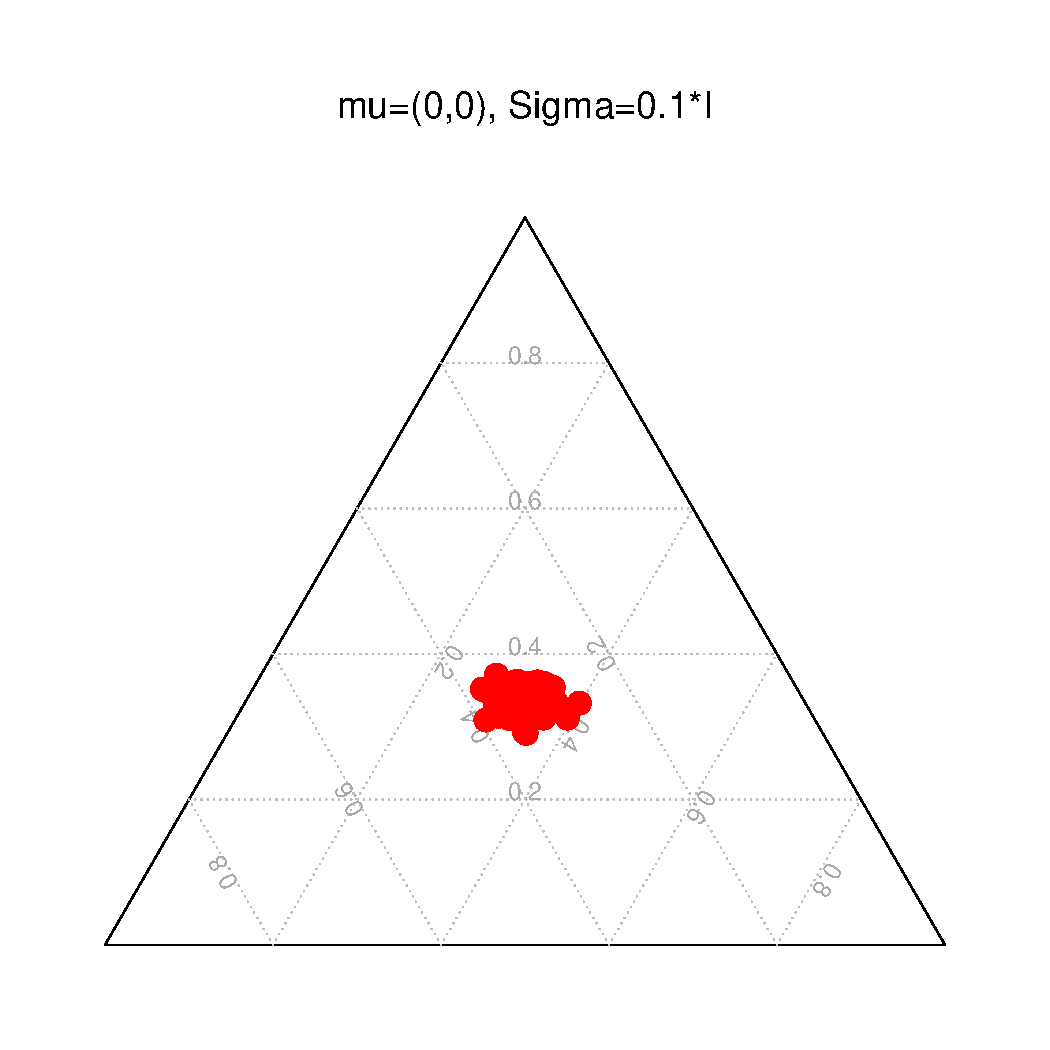
\includegraphics[width=\textwidth]{Sigma01_01.pdf}
\caption[ALN plot approximating the CGM model]{Here $\Sigma=0.1I$, and $\muvec=\vec{0}$, corresponds to roughly the CGM specification.}
\label{fig:figure8}
\end{minipage}
\end{figure}

 The simulations indicate that we can scale everything at approximately an $\mathcal{O}(d)$\newnot{symbol:big_oh} rate because of the diagonality of the variance covariance matrix, no matrix inversions are required. The step that remains is to link this portion of the model with the (currently) observed data in the tree, so that better trees are favored over trees that are worse, when each is observed in the Markov chain. We will first work in the space $\Rsp{d}$ and then translate to probabilities by using Equation \ref{eqn:simplex_transform}.  
 
 If we are to focus on the means and a collection of variances in a multivariate normal i.i.d. model, then we must fully specify the likelihood and the prior to form our posterior. 
 
 The likelihood of the tree is defined as follows: the tree's selected covariates are counted and summed across all observed splits, leading to a likelihood taking on discrete values for the observed data. Let us define a multiplier that can take on an arbitrary positive or negative value in a compact region. We then multiply the counts of splits on each covariate by this quantity, effectively creating a mean which can take on arbitrary values in $\Rsp{}$. 

\subsection{A Simple Sampler Approach}

This subsection derives the full conditional densities for each necessary update in the Gibbs loop to sample posterior weights on each dimension in the CGM decision tree sampler. 
 Throughout this subsection we will use the notation $\odot$\newnot{symbol:hadamard} to denote a Hadamard product of two matrices or vectors. 
 
 \subsubsection{The General Strategy}
 There are many problems with using a Dirichlet prior and a Multinomial conjugate likelihood. The two most glaring problems are the implicit prior assumption of same scales on each covariate and the fact that all covariances or, equivalently, correlations must be negative. If the generative model of the data is a linear model with an interaction term and a decision tree model is fit to the data, then several splits will occur on the two interacting covariates. These splits will occur alternately until the curvature is sufficiently approximated \cite{ishwaran2010high}. This situation indicates a positive correlation between the two covariates. Higher order interactions will result in similar positive correlations between collections of covariates. Therefore we conclude the Dirichlet density as a posterior for the probability of selecting a covariate is an inferior model. Moreover, the initial motivation for modeling data with a decision tree was to handle survey data that contained many complex interactions that would be too computationally expensive to evaluate using linear model methods \cite{morgan1963problems}. 
 
 The likelihood will be denoted by
 
 \begin{equation}\newnot{symbol:mvn}
 MVN(\vec{c}\odot\vec{s}\vert \vec{\mu}, \Sigma=\text{Diag}(\sigma^2_j)).
 \end{equation}
 
 The prior is also a normal 
 
 \begin{equation}
 \pi(\vec{\mu}\vert \vec{\mu}_p, \Sigma)=MVN(\vec{\mu}\vert \vec{\mu}_p, \Sigma).
 \end{equation}

The priors on the variances are \iid $\sim \invgam{\sigma_j^2}{a_j}{b_j}$.
Finally the priors on the $c_j$s are \iid\ scaled beta's with densities 

\begin{equation}\newnot{symbol:scaled_beta}
S\beta(c_j\vert \alpha_j, \beta_j, -a, a)\equiv\pi(c_j\vert \alpha_j, \beta_j, -a, a)= \frac{(c_j+a)^{\alpha_j-1}(a-c_j)^{\beta_j-1}\Gamma(\alpha_j+\beta_j)}{(2a)^{\alpha_j+\beta_j-1}\Gamma(\alpha_j)\Gamma(\beta_j)}.
\end{equation}

A special case of these scaled beta densities is when $\alpha_j=\beta_j=1$, which yields uniform r.v.'s on the region  $[-a,a]$. 
For each $j=1, \dots, d$, we first calculate $s_j = \epsilon+\sum_{\forall \eta \in \mathcal{T}}\mathds{1}[\text{split on covariate j at node $\eta$}]$, for some fixed $\epsilon>0$.
Through basic Bayesian calculations we find that the full conditionals are 

\begin{equation}
\pi(c_j\vert \mu_j, \sigma_j^2, a) \sim N_{[-a,a]}(c_js_j\vert \mu_j, \sigma^2_j) \text{(a normal truncated to the region $(-a,a)$),}
\end{equation}

\begin{equation}
\pi(\sigma^2_j \vert \mu_j, c_j, a) \sim \invgam{\sigma_j^2}{2a_j+2}{\frac{(c_js_j-\mu_j)^2+ (\mu_j-\mu_j^p)^2+b_j}{2}}, \text{ and } 
\end{equation}

\begin{equation}
\pi(\mu_j\vert \mu_j^p, c_j, \sigma^2_j)\sim N[c_js_j+\mu_j^p, \sigma_j^2].
\end{equation}

Ideally we would like everything to be a Gibbs step. This can be accomplished numerically using numerical approximations to the cumulative density of the standard normal distribution, here denoted $\Phi$, and $\Phi^{-1}$, the quantile function of the standard normal cumulative density. \newnot{symbol:sncdf} However, we can accomplish this directly using the technique of parameter expansion set forth in Damien and Walker \cite{damien2001sampling}, which we review here for completeness. 
 
We begin with the joint density of two random variables 

\begin{equation}
f(x,y) \propto \mathds{1}[0, \exp{(-x^2/2)}](y).
\end{equation}
The marginal of $x$ is a standard normal density. Through elementary probability calculations we find 

\begin{equation}\newnot{symbol:unif}
f(y\vert X=x) \propto Unif(0, \exp{(-x^2/2)}).
\end{equation}
 and 
 
 \begin{equation}
f(x\vert Y=y) \propto Unif(-\sqrt{-2log(y)}, \sqrt{-2log(y)})
\end{equation}
 The region upon which $X$ is defined arises from the solution of the inequalities $\{0\leq y \leq \exp{(-x^2/2)} \} $ for $X$, which is a quadratic equation in $X$. Similarly, if we have a truncated distribution truncated to the region $[a,b]$, we write the joint density 
 
 \begin{equation}
 f(x,y)=Unif((0\leq y\leq \exp{(-x^2/2)})\times (a,b)).
 \end{equation}
 Solving the resulting system of inequalities leads to the set 
 
 \begin{equation}
 \{-\sqrt{-2log(y)}, \sqrt{-2log(y)} \} \cap \{a, b\},
 \end{equation}
which results in the region for $x$

\begin{equation}
 \{\text{max}(a,-\sqrt{-2log(y)}), \text{min}(b,\sqrt{-2log(y)} )\} .
 \end{equation}
 Simulating from a truncated normal is equivalent to simulating from two uniforms on the appropriate regions and evaluating a natural logarithm and a square root. 
 
 A special case of these scaled beta densities is when $\alpha_j=\beta_j=1$, which yields uniform random variables on the region $[-a,a]$. 
For each $j=1, \dots, d$, we first calculate $s_j = \epsilon+\sum_{\forall \eta \in \mathcal{T}}\mathds{1}[\text{split on covariate j at node $\eta$}]$, for some fixed $\epsilon>0$.
Through basic Bayesian calculations we find the full conditionals in closed form
 
\begin{equation}\label{eqn:u_given_cjsj}
\pi(u \vert c_js_j, \mu_j, \sigma_j^2)= \text{Unif}(0, \exp{(\frac{-(c_js_j-\mu_j)^2}{2\sigma_j^2} )}),
\end{equation}

\begin{equation}
\pi(c_j \vert u) = \text{Unif}(\text{max}(-a,-\sqrt{-2log(u)}), \text{min}(a,\sqrt{-2log(u)} )),
\end{equation}

\begin{equation}
\pi(\sigma^2_j \vert \mu_j, c_j, a) \sim \invgam{\sigma_j^2}{2a_j+2}{\frac{(c_js_j-\mu_j)^2+ (\mu_j-\mu_j^p)^2+b_j}{2}}, \text{ and}
\end{equation}

\begin{equation}\label{eqn:muj_given_cj}
\pi(\mu_j\vert \mu_j^p, c_j, \sigma^2_j)\sim N[c_js_j+\mu_j^p, \sigma_j^2].
\end{equation}

 The Gibbs sampling step, nested within the MH sampler, proceeds by sampling from Equations \ref{eqn:u_given_cjsj}-\ref{eqn:muj_given_cj}
At each iteration, once samples are drawn in sequence from the distributions given in Equations \ref{eqn:u_given_cjsj}- \ref{eqn:muj_given_cj}, we take the posterior samples of $\mu_j$ and transform these onto the $[0,1]$ scale, by using the ALN transform given in Equation \ref{eqn:simplex_transform}. 

We show results from a preliminary coding of the stated algorithm. We use two specificications for the prior means $\vec{\mu}^p$. One specification uses  $\vec{\mu}^p = \vec{0}$ (Figure \ref{fig:simple_sampler2}) and another uses $\vec{\mu}^p=(-2,-2,2,\dots,2)$ (Figure \ref{fig:simple_sampler1}). The difference in the results of sampled weights indicates that, if we can move from a negative to a positive value for the prior mean, we can greatly influence the selection of covariates. The graphic of posterior weights shown in Figure \ref{fig:simple_sampler1} is the correct set of weights for the data. 


%%%% -------Graphics from preliminary simulations using the simple sampler approach

 \begin{figure}[ht]
\begin{minipage}[b]{0.45\linewidth}
\centering
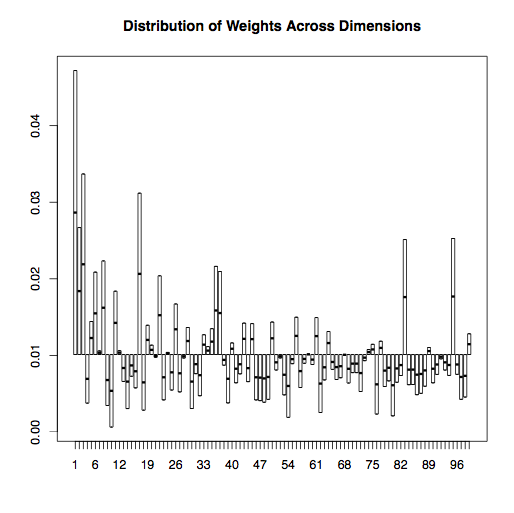
\includegraphics[scale=0.4]{simple_sampler2.png}
\caption[Results for the zero mean prior]{A zero mean prior. Note that the two covariates that should have large probabilities are covariates 1 and 2.}
\label{fig:simple_sampler2}
\end{minipage}
\hspace{0.5cm}
\begin{minipage}[b]{0.45\linewidth}
\centering
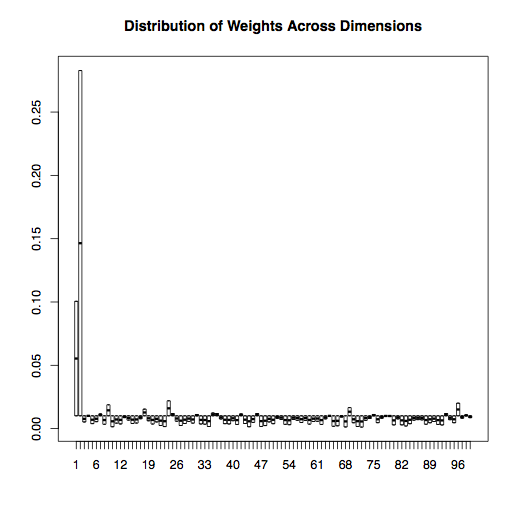
\includegraphics[scale=0.4]{simple_sampler1.png}
\caption[Results for the informative prior]{An informative prior. The first two prior means are 2 and the remaining prior means are set at -2.}
\label{fig:simple_sampler1}
\end{minipage}
\end{figure}


%%%%---------END OF: Graphics from preliminary simulations using the simple sampler approach

\subsection{A Stochastic Search Variable Selection Approach}

Using the results of George and McCulloch we can derive Gibbs updates for each of the parameters and have as a special case the approach of CGM if all the dimension indicators are selected to be the point masses at zero. In this case the ALN transform puts probability $1/(d+1)$ on each dimension. 


We investigate several priors for use in variable selection with decision trees. They are: 

\begin{itemize}
\item A stochastic search approach (method of George and McCulloch and Cui and George) \cite{cui2008empirical,george1993variable}. 
\item A lasso prior on the means of the MVN, \newabbrev{abbrev:MVN} probably using parameter expansion to get Gibbs updates \cite{park2008bayesian}. 
\item A multivariate half-Cauchy prior using parameter expansion (Huang and Wand method) \cite{huang2013simple,polson2011half,carvalho2010horseshoe,carvalhohandling}. 
\item A `local' prior approach (Valen Johnson and David Rossell JRSS B 2010 approach) \cite{johnson2010use}. 
\end{itemize}

We will discuss the preliminary details of each method in sequence in this chapter. 
%\textbf{Primary contributions of this research chapter:}

Variable selection with SSVS facilitates a Bayesian approach to variable selection in decision trees. Prior methods have examined bootstrapping approaches and used some complicated math to allow the statistician to peer inside the black box method known as randomForest \cite{ishwaran2010high, ishwaran2007variable}, often with little insight or understanding. The SSVS prior allows us to ``test'' whether the constant prior probability of selecting a covariate for all dimensions is appropriate for the given dataset. This means we can test, for any dataset, whether the CGM model of covariate selection is appropriate.
%In addition we receive an explicit measure of which covariates are important, something not achieved bagging , bumping or boosting \cite{breiman1996bagging, tibshirani1999model, freund1999short}. 

We will implement and compare our method against other methods such as observed frequency, a na\"{i}ve method, as well as the maximal subtree approach of Ishwaran et al. \cite{ishwaran2010high, ishwaran2007variable}. The SSVS approach involves a prior on the normal means of the form 

\begin{equation}
\pi(\mu_i\vert \tau_i, p_i, c_i) \propto p_iN(\mu_i, \tau_i^2)+(1-p_i)N(\mu_i, c_i^2\tau_i^2).
\end{equation}

Here the $c_i >1$ and $1>\tau_i>0$ is small. Usually $p_i\equiv1/2$ but it is also possible to put a prior on these hyper-parameters. The advantage of a mixture prior in this form is that Gibbs samples are readily available for each of the desired quantities facilitating fast sampling.     

What needs to be done for this approach is a couple of things: 

\begin{itemize}
\item Determine posteriors using these forms of priors. 
\item Determine if Gibbs sampling can be done on the resulting posteriors if priors for $p_i$ and/or $c_i$ and $\tau_i$ are used. 
\item Determine if a Beta prior on $p_i$ is computationally feasible.  
\item Extensive simulation studies and hyper-parameter sensitivities.
\end{itemize}
Plus any suggestions from the committee.

\subsection{A Lasso Prior}
In this section we propose to use parameter expansion to facilitate Gibbs sampling within the sampling framework for the posterior means for each covariate in the normal space. We use the ALN transform to then convert to probabilities. 
The key idea we use for parameter expansion is the scale mixture of normals representation of a Laplace prior. This representation is stated here for reference.

If $V \sim \text{Exponential(1)}$ and $Z \sim N(0, 1)$ independent of $V$, then $X = \mu + b \sqrt{2 V}Z \sim \mathrm{Laplace}(\mu,b)$. 

Equivalently we can write this as the hierarchy

\begin{equation}\label{eqn:normal_cond_lhood_lasso}
X \vert V \sim N[\mu, \sigma^22V],
\end{equation}

\begin{equation}\newnot{symbol:exponential_dist}
V \sim \text{Exponential}(1), \text{ and}
\end{equation}

\begin{equation}\newnot{symbol:laplace_dist}
X \sim \text{Laplace}(\mu, \sigma)
\end{equation}

What we want to examine here is whether shrinkage along an $L_1$ penalty will achieve similar results to the SSVS approach and give us meaningful results. The belief here is the same as in the SSVS approach, shrinkage will shrink means toward zero in the multivariate normal. These sampled values from the multivariate normal will then be transformed into something on the $[0,1]$ (probability) scale using the ALN transform. Values of zero, or near zero, on the normal space transform into values of approximately $1/(d+1)$. The probabilities with values around $1/(d+1)$ correspond to covariates we are indifferent about. A confounding aspect of interpreting the probabilities is that they must all sum to 1. Therefore if some values are excessively small this may push all the other probabilities to be larger. If something like this happens it is then difficult to determine which covariates are non-informative. Further simulations regarding selecting covariates using the rule of Equation \ref{eqn:cov_inclusion_rule} will be conducted using the ALN transform and will be done on several simulated and real data examples.    

What needs to be done for this approach is a couple of things: 

\begin{itemize}
\item Write out the full conditionals and the Gibbs samplers for this case. 
\item Code the full conditional sampler for this method. 
\item Compare parameterizations and evaluate the sensitivity to hyper-parameter specifications. 
\item Extensive simulation studies. 
\end{itemize}
Also any suggestions by the committee.
\subsection{A Half-Cauchy or Horseshoe Prior}

The following result will be useful for parameter expansion. If 

$X\vert a \sim \mathrm{Inv-Gamma}(\nu/2, \nu/a)$ and  $a \sim \mathrm{Inv-Gamma}(1/2,A^2)$, then $\sqrt{X}\sim \mathrm{Half-Cauchy}$. 

\begin{align*}
f(x) &= \int_0^\infty \underbrace{  \frac{\nu^{\nu/2}}{a^{\nu/2}\Gamma(\nu/2)x^{(\nu/2)+1}}\exp{(-\frac{\nu}{ax})}   }_{=f(x\vert a)} \underbrace{\frac{\exp{(-\frac{1}{aA^2})}}{A\sqrt{\pi}a^{3/2}}}_{=f(a)} da\\
&=\frac{\nu^{\nu/2}}{A\sqrt{\pi}\Gamma(\nu/2)x^{(\nu+2)/2}}\underbrace{\int_0^\infty a^{-\nu/2-1/2-1}\exp{(-(1/a)(\nu/x+1/A^2))}da}_{=\text{Inv-Gamma kernel}}\\
&=\frac{\nu^{\nu/2}\Gamma((\nu+1)/2)}{A\sqrt{\pi}\Gamma(\nu/2)x^{(\nu+2)/2}(\nu/x+1/A^2)^{(\nu+1)/2}}\\
&\propto \frac{1}{\sqrt{x}x^{(\nu+1)/2}(\nu/x+1/A^2)^{(\nu+1)/2}}\\
& =\frac{1}{\sqrt{x}(\nu+x/A^2)^{(\nu+1)/2}  }\\
&=\frac{1}{\sqrt{x}(\nu+x/A^2)^{(\nu+1)/2}  }.
\end{align*}

Making the change of variable $x=y^2$, which implies $dx/(2\sqrt{x})=dy$, shows us that 

\begin{equation}
f(y) \propto (1+(y/A)^2/\nu)^{-(\nu+1)/2},
\end{equation}
for $y>0$ which is the definition of a half-Cauchy density. 

Huang and Wand \cite{huang2013simple} indicate that using an inverse-Wishart prior on the variances, with each standard deviation having a half-Cauchy prior, gives a scaled beta marginal for each correlation. At this point it is worth recalling that the t and half-t distributions have as special cases, the Cauchy and half-Cauchy distributions when the degrees of freedom parameter ($\nu$) in the t and half-t is set to $\nu=1$. We will use the scale mixture representation of inverse gammas given above to put half-Cauchy priors on the standard deviations.  


%%%% Leave this chunk in for now, but will probably cut it in the end
The hierarchical model for the sparse inverse-Wishart prior as

\begin{equation}\newnot{symbol:inv_wishart}
\Sigma\vert a_1, \dots,a_p \sim \text{Inv-Wishart}(\nu+p-1, 2\nu\text{diag}(1/a_1,\dots,1/a_p)), 
\end{equation} 

\begin{equation}
a_k \sim i.i.d.\ \text{Inverse-Gamma}(1/2,1/A_k^2),
\end{equation} 
for $k=1,\dots,p$.  
The inverse-Wishart has the density 
\begin{equation}
p(\Sigma \vert \kappa, \text{B})\propto \vert \text{B}\vert^{\kappa/2}\vert\Sigma\vert^{-(\kappa+p+1)/2}\exp{(-\frac{1}{2}\text{tr}(B\Sigma^{-1}))}.
\end{equation}
\newnot{symbol:trace}
Huang and Wand \cite{huang2013simple} argue that this model constitutes a matrix generalization of the half-t$(\nu, A_k)$ prior for each standard deviation term, and also allows for uniform marginal distributions on each correlation parameter in $\Sigma$, by choosing $\nu=2$. If one instead chooses $\nu=1$, this corresponds to a $S\beta(\rho;1/2,1/2,-1,1)$ distribution. This half-t prior works well in their simulations for both correlated covariates and non-correlated covariates.  
%%%% End of this chunk in for now, but will probably cut it in the end
What needs to be done for this method is: 

\begin{itemize}
\item Write down full conditionals.
\item Code the full conditionals samplers. 
\item Determine the dimensionality in which this method is feasible and if that is useful for our problems.
\item Extensive simulation studies. 
\end{itemize}
Also, any suggestions that committee brings up during the proposal.

%\subsection{A Local Prior Approach}
%
%Another alternative we will examine is a `local' prior approach using a moment prior defined in Johnson and Rossell \cite{johnson2010use}. These moment priors are functions that have densities that look like those in Figure \ref{fig:local_priors}.
%
%\begin{figure}[h]
%  \centering
%    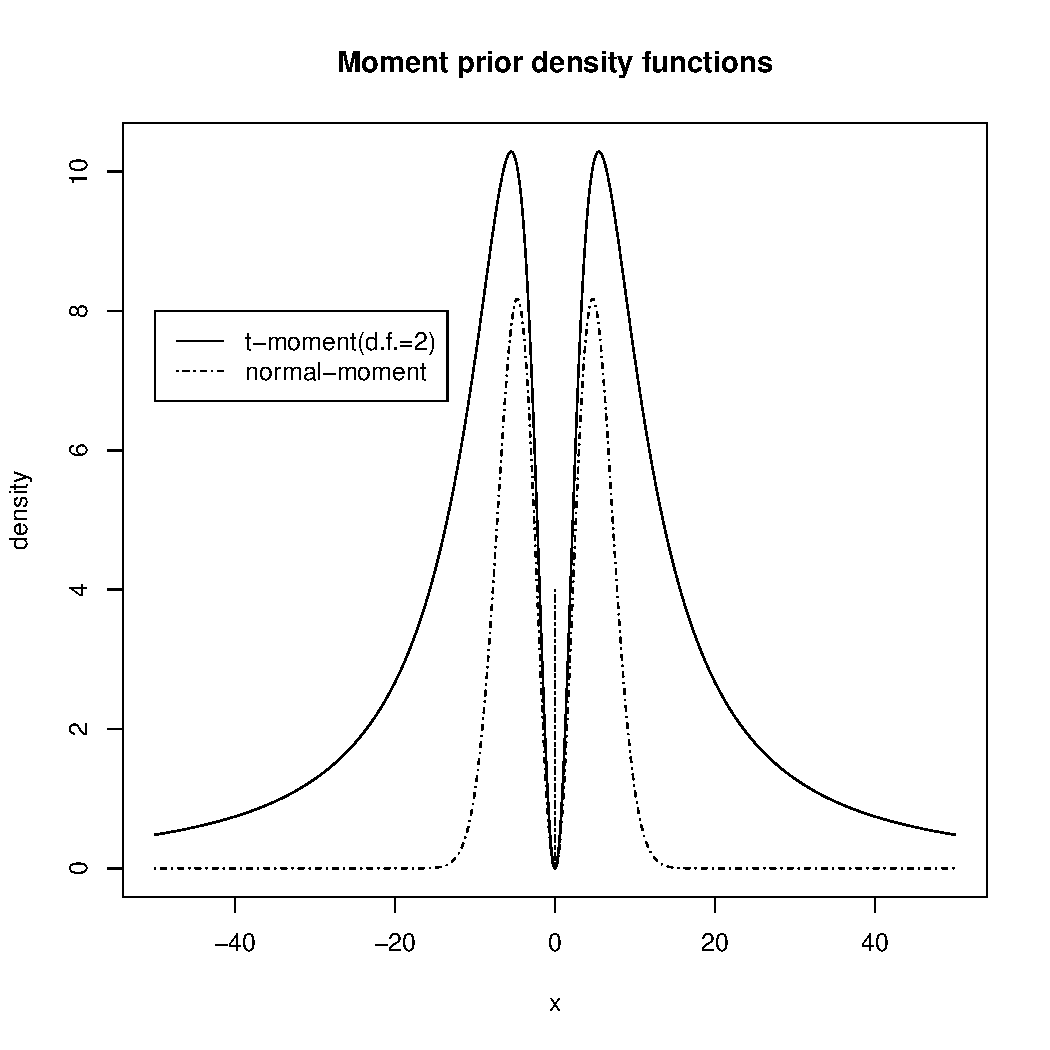
\includegraphics[width=0.7\textwidth]{moment_prior_plot_BW.pdf}
%    \caption[Local priors with a point mass at 0]{Local priors with a point mass at 0.}
%  \label{fig:local_priors}
%\end{figure}
%
%The moment priors are defined by the densities 
%
%\begin{equation}
%f_k(x)\propto (x-\mu)^{2k}\pi(x-\mu),
%\end{equation}
%where here $\mu$ denotes the first moment and $k$ is a specified constant. In Figure \ref{fig:local_priors} $k=1$, $\mu=0$, and the two $\pi(x)$s represent a normal and a t distribution with degrees of freedom $2$. The basic idea with the local priors is that we want to circumvent the necessity of specifying informative prior means for the normal priors. These moment priors have large probability masses on two regions, a negative region and a positive region. The two local modes allow the priors' means to encourage the selection of certain covariates (in the positive mode) and to discourage the selection of other covariates (in the negative mode).
%
%What needs to be done for this approach is extensive simulation studies and hyper-parameter sensitivities.
%
%Also, any suggestions that committee brings up during the proposal.



